%!TEX TX-program = xelatex
\documentclass[8pt]{article}
\usepackage{allan-eason}

\usetikzlibrary{positioning}
\usetikzlibrary{svg.path}

\graphicspath{ {./images/} }

\newcommand{\Date}{220427}
\newcommand{\Test}{反三角与向量}

\newcommand{\Author}{Eason S.}
\newcommand{\Title}{\textcolor{allandarkblue}{\Date}\ \textcolor{allancyan}{\Test}\ 题目选解}

\author{\Author}
\title{\Title}
\date{}

\geometry{a4paper, scale=0.8}

\lhead{\Title}

\begin{document}

	\maketitle

	\section{填空题}
		\defword{1.} 下列各式正确的是 \answord{(1) (3)}.

		\begin{multicols}{2}
			\begin{enumerate}[label=\calword{(\arabic*)}]
				\item \(\displaystyle \arcsin \left(\sin \frac{5\pi}{4}\right) = -\frac{\pi}{4}\);
    			\item \(\displaystyle \arcsin \left(- \frac{\pi}{3}\right) = -\frac{\sqrt{3}}{2}\);
       			\item \(\displaystyle \arccos \left(- \frac{\sqrt{3}}{2}\right) = \frac{5\pi}{6}\);
          		\item \(\displaystyle \sin \left(\arcsin \frac{\pi}{3}\right) = \frac{\pi}{3}\);
				\item \(\displaystyle \sin \left[\arccos \left(-\frac{1}{2}\right)\right] = -\frac{\sqrt{3}}{2}\).
			\end{enumerate}
		\end{multicols}

		\answord{解析.} 反三角函数.

		\defword{2.} 方程\(\sin x = \lg x\)的实根有 \answord{3} 个.
		
		\answord{解析.} 可通过函数图像判断方程解的个数的超越方程.

		\(\lg x = 1 \Iff x = 10 > 3\pi,\)

		\[
		\begin{tikzpicture}
			\draw[black, ->] (-1, 0)--({3 * pi + 1}, 0) node[above] {\(x\)};
			\draw[black, ->] (0, -2)--(0, 2) node[right] {\(y\)};
			\draw[black, domain = 0:{3 * pi}, samples = 1000] plot(\x,{sin deg \x});
			\draw[black, domain = 0.1:{3 * pi}, samples = 1000] plot(\x,{(ln \x) / (ln 10)});
		\end{tikzpicture}
		\]

		\defword{3.} 满足 \(\arccos 2x < \arccos (1-x)\)的\(x\)的取值集合为 \answord{\(\left(\dfrac{1}{3}, \dfrac{1}{2}\right]\)}.
		
		\answord{解析.} 可化为代数不等式的三角不等式.
		
		\defword{4.} 已知\(A(0, 3), B(2, 0), C(-1, 3)\)与\(\ray{AB} + 2\ray{AC}\)方向相反的单位向量是 \answord{\((0, 1)\)}.
		
		\answord{解析.} 向量的基本运算.

		\defword{5.} 在\(\triangle ABC\)中, \(a = 5, b = 8, C = 60\degree\), 则\(\ray{BC} \cdot \ray{CA}\)的值为 \answord{\(-20\)}.
		
		\answord{解析.} 向量的基本运算, 三角形.

		\defword{6.} 设函数\(y = \arctan x\)的图像沿\(x\)轴正方向平移\(2\)个单位, 所得图像为\(C_1\), 又设图像\(C_2\)与\(C_1\)关于原点对称, 那么\(C_2\)所对应的函数是 \answord{\(y = \arctan(x+2)\)}.
		
		\answord{解析.} 函数的变换.

		\begin{center}
			\begin{tabular}{rcl}
				\(y = \arctan x\) 	& \(\xlongrightarrow{\text{向右平移\(2\)个单位}}\) & \(y = \arctan (x-2)\)\\
								& \(\xlongrightarrow{\text{关于原点对称}}\) & \(-y = \arctan (-x - 2)\)\\
								& \(\Rightarrow\) & \(y = \arctan (x + 2)\).
			\end{tabular}
		\end{center}

		\defword{7.} 函数\(y = 2\arcsin 3x \left(0 < x \leq \dfrac{1}{3}\right)\)的值域为 \answord{\((0, \pi]\)}.
		
		\answord{解析.} 反三角函数.

		\defword{8.} 方程\(\sin 3x - \sin x = 0\)的解集是 \answord{\(\left\{x | x = k\pi \lgor x = \dfrac{2k+1}{4}\pi, k \in \ZZ\right\}\)}.
		
		\answord{解析.} 可化为代数方程的三角方程.

		\begin{align*}
			\sin 3x - \sin x = 0	& \Rightarrow \sin 3x = \sin x \\
									& \Rightarrow 3x = x + 2k\pi \lgor 3x = \pi - x + 2k\pi, k \in \ZZ\\
									& \Rightarrow x = k\pi \lgor 4x = \pi + 2k\pi, k \in \ZZ\\
									& \Rightarrow x = k\pi \lgor x = \dfrac{2k+1}{4}\pi, k \in \ZZ.
		\end{align*}

		\defword{9.} 函数\(y = \sin x, x \in \left[\dfrac{\pi}{2}, \dfrac{3\pi}{2}\right]\)的反函数为 \answord{\(y = \pi - \arcsin x, x \in [-1, 1]\)}.
		
		\answord{解析.} 反三角函数.

		\defword{10.} 方程 \(\sqrt{5\cos x + \cos 2x} + \sin x = 0\)在\([0, 2\pi]\)上的解集是 \answord{\(\left\{2\pi - \arccos \dfrac{1}{3}\right\}\)}.
		
		\answord{解析.} 三角方程.

        \begin{align*}
            \sqrt{5\cos x + \cos 2x} + \sin x = 0, x \in [0, 2\pi] & \Rightarrow 5\cos x + \cos 2x = \sin^2 x \lgand \sin x \leq 0 \lgand x \in [0, 2\pi]\\
            & \Rightarrow 5\cos x + 2\cos^2 x - 1 = 1 - \cos^2 x, x\in [\pi, 2\pi]\\
            & \Rightarrow 2\cos^2 x + 5\cos x - 2 = 0, x\in [\pi, 2\pi]\\
            & \Rightarrow (3\cos x - 1)(\cos x + 2) = 0, x\in [\pi, 2\pi]\\
            & \Rightarrow \cos x = \frac{1}{3} \lgor \cos x = -2, x\in [\pi, 2\pi]\\
            & \Rightarrow x = \pm \arccos \frac{1}{3} + 2k\pi, k\in \ZZ \lgand x\in [\pi, 2\pi]\\
            & \Rightarrow x = 2\pi - \arccos \frac{1}{3}.
        \end{align*}
		
		\defword{11.} 在 \(\triangle ABC\)中, \(AB = 2, BC = 3, \angle ABC = 60\degree, AD\)为\(BC\)边上的高, \(O\)为\(AD\)的中点, 若\(\ray{AO} = \lambda \ray{AB} + \mu \ray{BC},\)其中\(\lambda, \mu \in \RR\), 则\(\lambda + \mu\)等于 \answord{\(\dfrac{2}{3}\)}.

		\answord{解析.} 向量的线性组合.

        显然有

        \[\ray{AD} = \ray{AB} + \ray{BD} = \ray{AB} + \frac{1}{6} \ray{BC},\]

        又\(O\)为\(AD\)中点, 有

        \[\ray{AO} = \frac{1}{2} \ray{AD} = \frac{1}{2} \ray{AB} + \frac{1}{6} \ray{BC}, \]

        于是有\(\lambda = \dfrac{1}{2}, \mu = \dfrac{1}{6}, \lambda + \mu = \dfrac{2}{3}\).
		
		\defword{12.} 如图, 菱形\(ABCD\)的边长为\(2\), \(\angle BAD = 60\degree\), \(M\)为\(DC\)的中点, 若\(N\)为菱形内任意一点 (含边界), 则\(\ray{AM} \cdot \ray{AN}\)的最大值为 \answord{\(9\)}.

		\answord{解析.} 向量几何综合.

        \[
		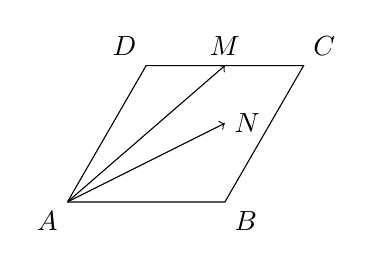
\begin{tikzpicture}
			\draw[black] (0, 0)--(2, 0)--(3, {sqrt(3)})--(1, {sqrt(3)})--(0, 0) node at (0, 0) [anchor = north east] {\(A\)} node at (2, 0) [anchor = north west] {\(B\)} node at (3, {sqrt(3)}) [anchor = south west] {\(C\)} node at (1, {sqrt(3)}) [anchor = south east] {\(D\)} node at (2, {sqrt(3)}) [anchor = south] {\(M\)};
            \draw[black, ->] (0, 0)--(2, {sqrt(3)});
            \draw[black, ->] (0, 0)--(2, 1) node [right] {\(N\)};
		\end{tikzpicture}
		\]

        由向量的内积的定义, 有

        \[\ray{AM} \cdot \ray{AN} = \abs{\ray{AM}} \Prj{\ray{AM}}{\ray{AN}},\]

        于是有
        
        \begin{align*}
            \max \left(\ray {AM} \cdot \ray{AN}\right)    &= \ray{AM} \cdot \ray{AC}\\
                                                            &= \left(\frac{1}{2}\ray{AB} + \ray{AD}\right) \cdot \left(\ray{AB} + \ray{AD}\right)\\
                                                            &= \frac{1}{2} \ray{AB}^2 + \ray{AD}^2 + \frac{3}{2} \ray{AB} \cdot \ray{AD}\\
                                                            &= 9.
        \end{align*}

	\section{解答题}
		\defword{13.} 已知函数\(f(x) = \sqrt{3} \cos^2 x + \sin x \cos x, x \in [0, \pi]\),
			\begin{enumerate}[label=\calword{(\arabic*)}]
				\item 求函数\(f(x)\)的单调递增区间. \answord{\(\left[0, \dfrac{\pi}{12}\right], \left[\dfrac{7\pi}{12}, \pi\right]\)}.

					\answord{解析.} 三角函数的单调性.

                    \[f(x) = \sqrt{3} \cos^2 x + \sin x \cos x = \sin \left(2x + \frac{\pi}{3}\right) + \frac{\sqrt{3}}{2}.\]

				\item 如果关于\(x\)的方程\(\abs{f(x)} = m\), 在区间\((0, \pi)\)上有两个不同的实根, 求实数\(m\)的取值范围. \answord{\(m \in \{0\}\cup\left(1-\dfrac{\sqrt{3}}{2}, \sqrt{3}\right)\cup\left(\sqrt{3}, 1+\dfrac{\sqrt{3}}{2}\right)\)}.
    
					\answord{解析.} 利用图像解方程.

                    \[
                        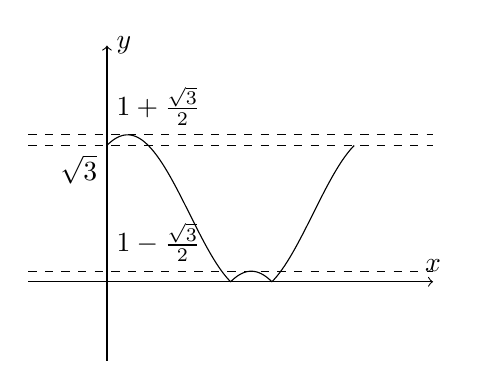
\begin{tikzpicture}
                            \draw[black, ->] (-1, 0)--({pi + 1}, 0) node[above] {\(x\)};
                            \draw[black, ->] (0, -1)--(0, 3) node[right] {\(y\)};
                            \draw[black, domain = 0:{pi}, samples = 1000] plot(\x,{abs(sin deg (2 * \x + pi / 3) + sqrt(3) / 2)});
                            \draw[black, dashed] (-1, {1 + sqrt(3) / 2})--({pi + 1}, {1 + sqrt(3) / 2}) node at (0, {1 + sqrt(3) / 2}) [anchor = south west] {\(1 + \frac{\sqrt{3}}{2}\)};
                            \draw[black, dashed] (-1, {sqrt(3)})--({pi + 1}, {sqrt(3)}) node at (0, {sqrt(3)}) [anchor = north east] {\(\sqrt{3}\)};
                            \draw[black, dashed] (-1, {1 - sqrt(3) / 2})--({pi + 1}, {1 - sqrt(3) / 2}) node at (0, {1 - sqrt(3) / 2}) [anchor = south west] {\(1 - \frac{\sqrt{3}}{2}\)};
                        \end{tikzpicture}
                    \]

			\end{enumerate}
		
		\defword{14.} 甲船在\(A\)处观察到乙船在它的北偏东\(60 \degree\)方向的\(B\)处, 两船相距\(a\)海里, 乙船正向北行驶, 若甲船是乙船速度的\(\sqrt{3}\)倍, 问甲船应取什么方向前进才能在最短时间内追上乙船? 此时乙船行驶多少海里? \answord{北偏东\(30\degree\); \(a\)海里}.

		\answord{解析.} 太水了, 不写.
		
		\defword{15.} 已知\(\vec{a} = \left(\cos \alpha, \sin \alpha\right), \vec{b} = \left(\cos \beta, \sin \beta\right)\), 其中\(0 < \alpha < \beta < \pi\),
			\begin{enumerate}[label=\calword{(\arabic*)}]
				\item 求证: \(\vec{a} + \vec{b}\)与\(\vec{a} - \vec{b}\)互相垂直.
					
					\answord{解析.} 向量垂直 (正交) \(\Leftrightarrow\) 内积为\(0\).
				\item 若\(k \vec{a} + \vec{b}\)与\(\vec{a} - k\vec{b}\)的长度相等, 求\(\beta - \alpha\)的值, 其中\(k \in \RR \setminus \{0\}\). \answord{\(\dfrac{\pi}{2}\)}.

					\answord{解析.} 向量的模相等 \(\Leftrightarrow\) 向量的模的平方相等 \(\Leftrightarrow\) 向量与自身的内积相等.

                    \begin{align*}
                        \abs{k \vec{a} + \vec{b}} = \abs{\vec{a} - k \vec{b}} &\Rightarrow \abs{k \vec{a} + \vec{b}}^2 = \abs{\vec{a} - k \vec{b}}^2 \\
                        &\Rightarrow \left(k\vec{a} + \vec{b}\right)^2 = \left(a - k \vec{b}\right)^2\\
                        &\Rightarrow k^2 \abs{\vec{a}}^2 + 2k\vec{a} \cdot \vec{b} + \abs{\vec{b}}^2 = \abs{\vec{a}}^2 - 2k\vec{a} \cdot \vec{b} + k^2 \abs{\vec{b}}^2.
                    \end{align*}

                    有\(\abs{\vec{a}} = \abs{\vec{b}} = 1\), 有

                    \[k^2 + 2k\vec{a} \cdot \vec{b} + 1 = 1 - 2k\vec{a} \cdot \vec{b} + k^2,\]

                    有

                    \[\vec{a} \cdot \vec{b} = 0,\]

                    即

                    \[(\cos \alpha, \sin \alpha) \cdot (\cos \beta, \sin \beta) = 0,\]

                    即

                    \[\cos \alpha \cos \beta + \sin \alpha \sin \beta = 4 \cos (\beta - \alpha) = 0.\]

                    因为有\(0 < \alpha < \beta < \pi\), 有\(\beta - \alpha = \dfrac{\pi}{2}\).

			\end{enumerate}

	\section{附加题}
		\defword{16.} 在\(\triangle ABC\)中, \(\ray{AB} \cdot \ray{AC} = \abs{\ray{AB} - \ray{AC}} = 2\).
			\begin{enumerate}[label=\calword{(\arabic*)}]
				\item 求\(\abs{\ray{AB}}^2 + \abs{\ray{AC}}^2\)的值. \answord{\(8\)}.
    
					\answord{解析.} 向量的基础应用.

                    显然有

                    \[\abs{\ray{AB}}^2 + \abs{\ray{AC}}^2 - 2\ray{AB}\cdot\ray{AC} = 4,\]

                    即

                    \[\abs{\ray{AB}}^2 + \abs{\ray{AC}}^2 = 2 \ray{AB} \cdot \ray{AC} + 4,\]

                    又\(\ray{AB} \cdot \ray{AC} = 2\), 有

                    \[\abs{\ray{AB}}^2 + \abs{\ray{AC}}^2 = 8.\]

				\item 当\(\triangle ABC\)的面积最大时, 求\(\angle A\)的大小. \answord{\(\dfrac{\pi}{3}\)}.
    
					\answord{解析.} 三角形面积公式, 同角三角比.

                    由向量的内积的定义, 有\(\cos \angle BAC = \dfrac{2}{\abs{\ray{AB}} \cdot \abs{\ray{AC}}}\), 有
                    
                    \[\sin \angle BAC = \sqrt{1 - \left(\frac{2}{\abs{\ray{AB}}\cdot\abs{\ray{AC}}}\right)^2}=\frac{\sqrt{\left(\abs{\ray{AB}}\cdot\abs{\ray{AC}}\right)^2 - 4}}{\abs{\ray{AB}} \cdot \abs{\ray{AC}}}.\]

                    由三角形正弦面积公式

                    \begin{align*}
                        S_{\triangle ABC}   &= \frac{1}{2} \abs{\ray{AB}} \cdot \abs{\ray{AC}} \sin \angle BAC\\
                                            &= \frac{1}{2} \sqrt{\left(\abs{\ray{AB}} \cdot \abs{\ray{AC}}\right)^2 - 4}\\
                                            &\leq \frac{1}{2} \sqrt{\left(\frac{\abs{\ray{AB}} + \abs{\ray{AC}}}{2}\right)^4 - 4},
                    \end{align*}

                    等号成立当且仅当\(\abs{\ray{AB}} = \abs{\ray{AC}} = 2,\) 即\(\cos \angle BAC = \dfrac{1}{2}\), 即\(\angle BAC = \dfrac{\pi}{3}\).

			\end{enumerate}
\end{document}